% Options for packages loaded elsewhere
\PassOptionsToPackage{unicode}{hyperref}
\PassOptionsToPackage{hyphens}{url}
\PassOptionsToPackage{dvipsnames,svgnames,x11names}{xcolor}
\documentclass[
  12pt,
]{scrreprt}
\usepackage{xcolor}
\usepackage[margin=1in]{geometry}
\usepackage{amsmath,amssymb}
\setcounter{secnumdepth}{5}
\usepackage{iftex}
\ifPDFTeX
  \usepackage[T1]{fontenc}
  \usepackage[utf8]{inputenc}
  \usepackage{textcomp} % provide euro and other symbols
\else % if luatex or xetex
  \usepackage{unicode-math} % this also loads fontspec
  \defaultfontfeatures{Scale=MatchLowercase}
  \defaultfontfeatures[\rmfamily]{Ligatures=TeX,Scale=1}
\fi
\usepackage{lmodern}
\ifPDFTeX\else
  % xetex/luatex font selection
  \setmainfont[]{Garamond}
  \setsansfont[]{Gotham-Book.otf}
  \setmonofont[]{Courier New}
\fi
% Use upquote if available, for straight quotes in verbatim environments
\IfFileExists{upquote.sty}{\usepackage{upquote}}{}
\IfFileExists{microtype.sty}{% use microtype if available
  \usepackage[]{microtype}
  \UseMicrotypeSet[protrusion]{basicmath} % disable protrusion for tt fonts
}{}
\makeatletter
\@ifundefined{KOMAClassName}{% if non-KOMA class
  \IfFileExists{parskip.sty}{%
    \usepackage{parskip}
  }{% else
    \setlength{\parindent}{0pt}
    \setlength{\parskip}{6pt plus 2pt minus 1pt}}
}{% if KOMA class
  \KOMAoptions{parskip=half}}
\makeatother
\usepackage{color}
\usepackage{fancyvrb}
\newcommand{\VerbBar}{|}
\newcommand{\VERB}{\Verb[commandchars=\\\{\}]}
\DefineVerbatimEnvironment{Highlighting}{Verbatim}{commandchars=\\\{\}}
% Add ',fontsize=\small' for more characters per line
\usepackage{framed}
\definecolor{shadecolor}{RGB}{248,248,248}
\newenvironment{Shaded}{\begin{snugshade}}{\end{snugshade}}
\newcommand{\AlertTok}[1]{\textcolor[rgb]{0.94,0.16,0.16}{#1}}
\newcommand{\AnnotationTok}[1]{\textcolor[rgb]{0.56,0.35,0.01}{\textbf{\textit{#1}}}}
\newcommand{\AttributeTok}[1]{\textcolor[rgb]{0.13,0.29,0.53}{#1}}
\newcommand{\BaseNTok}[1]{\textcolor[rgb]{0.00,0.00,0.81}{#1}}
\newcommand{\BuiltInTok}[1]{#1}
\newcommand{\CharTok}[1]{\textcolor[rgb]{0.31,0.60,0.02}{#1}}
\newcommand{\CommentTok}[1]{\textcolor[rgb]{0.56,0.35,0.01}{\textit{#1}}}
\newcommand{\CommentVarTok}[1]{\textcolor[rgb]{0.56,0.35,0.01}{\textbf{\textit{#1}}}}
\newcommand{\ConstantTok}[1]{\textcolor[rgb]{0.56,0.35,0.01}{#1}}
\newcommand{\ControlFlowTok}[1]{\textcolor[rgb]{0.13,0.29,0.53}{\textbf{#1}}}
\newcommand{\DataTypeTok}[1]{\textcolor[rgb]{0.13,0.29,0.53}{#1}}
\newcommand{\DecValTok}[1]{\textcolor[rgb]{0.00,0.00,0.81}{#1}}
\newcommand{\DocumentationTok}[1]{\textcolor[rgb]{0.56,0.35,0.01}{\textbf{\textit{#1}}}}
\newcommand{\ErrorTok}[1]{\textcolor[rgb]{0.64,0.00,0.00}{\textbf{#1}}}
\newcommand{\ExtensionTok}[1]{#1}
\newcommand{\FloatTok}[1]{\textcolor[rgb]{0.00,0.00,0.81}{#1}}
\newcommand{\FunctionTok}[1]{\textcolor[rgb]{0.13,0.29,0.53}{\textbf{#1}}}
\newcommand{\ImportTok}[1]{#1}
\newcommand{\InformationTok}[1]{\textcolor[rgb]{0.56,0.35,0.01}{\textbf{\textit{#1}}}}
\newcommand{\KeywordTok}[1]{\textcolor[rgb]{0.13,0.29,0.53}{\textbf{#1}}}
\newcommand{\NormalTok}[1]{#1}
\newcommand{\OperatorTok}[1]{\textcolor[rgb]{0.81,0.36,0.00}{\textbf{#1}}}
\newcommand{\OtherTok}[1]{\textcolor[rgb]{0.56,0.35,0.01}{#1}}
\newcommand{\PreprocessorTok}[1]{\textcolor[rgb]{0.56,0.35,0.01}{\textit{#1}}}
\newcommand{\RegionMarkerTok}[1]{#1}
\newcommand{\SpecialCharTok}[1]{\textcolor[rgb]{0.81,0.36,0.00}{\textbf{#1}}}
\newcommand{\SpecialStringTok}[1]{\textcolor[rgb]{0.31,0.60,0.02}{#1}}
\newcommand{\StringTok}[1]{\textcolor[rgb]{0.31,0.60,0.02}{#1}}
\newcommand{\VariableTok}[1]{\textcolor[rgb]{0.00,0.00,0.00}{#1}}
\newcommand{\VerbatimStringTok}[1]{\textcolor[rgb]{0.31,0.60,0.02}{#1}}
\newcommand{\WarningTok}[1]{\textcolor[rgb]{0.56,0.35,0.01}{\textbf{\textit{#1}}}}
\usepackage{graphicx}
\makeatletter
\newsavebox\pandoc@box
\newcommand*\pandocbounded[1]{% scales image to fit in text height/width
  \sbox\pandoc@box{#1}%
  \Gscale@div\@tempa{\textheight}{\dimexpr\ht\pandoc@box+\dp\pandoc@box\relax}%
  \Gscale@div\@tempb{\linewidth}{\wd\pandoc@box}%
  \ifdim\@tempb\p@<\@tempa\p@\let\@tempa\@tempb\fi% select the smaller of both
  \ifdim\@tempa\p@<\p@\scalebox{\@tempa}{\usebox\pandoc@box}%
  \else\usebox{\pandoc@box}%
  \fi%
}
% Set default figure placement to htbp
\def\fps@figure{htbp}
\makeatother
\setlength{\emergencystretch}{3em} % prevent overfull lines
\providecommand{\tightlist}{%
  \setlength{\itemsep}{0pt}\setlength{\parskip}{0pt}}
\usepackage[round,authoryear]{natbib}
\bibliographystyle{apalike}
% header.tex
\usepackage{graphicx}
\usepackage{titling}
\usepackage{fancyhdr}
\usepackage{fontspec}   % For loading fonts
\usepackage{xcolor}     % For color definitions
\usepackage{mdframed}
\usepackage{tocloft}    % For customizing the TOC

% Define the Boise State Blue color
\definecolor{boisestateblue}{HTML}{0033A0}

% Load Gotham fonts
\newfontface\gothamblack{Gotham-Black.otf}[Path=../Document_fonts/]
\newfontface\gothambold{Gotham-Bold_0.otf}[Path=../Document_fonts/]
\newfontface\gothambolditalic{Gotham-BoldItalic.otf}[Path=../Document_fonts/]
\newfontface\gothambook{Gotham-Book.otf}[Path=../Document_fonts/]
\newfontface\gothammedium{Gotham-Medium.otf}[Path=../Document_fonts/]

% Set the document's main font to Garamond
\setmainfont{Garamond}
% Set the sans-serif font (used for headings) to Gotham Book
\setsansfont{Gotham-Book.otf}[Path=../Document_fonts/]
% Set the monospace font to Garamond
\setmonofont{Garamond}

% -----------------------------------------------------------------------------
% Style the Table of Contents using tocloft + Gotham
% -----------------------------------------------------------------------------
\renewcommand{\cfttoctitlefont}{\Huge \sffamily \bfseries \color{boisestateblue}}
\renewcommand{\cftsecfont}{\normalfont\sffamily}
\renewcommand{\cftsecpagefont}{\normalfont\sffamily}
\renewcommand{\cftsubsecfont}{\normalfont\sffamily}
\renewcommand{\cftsubsecpagefont}{\normalfont\sffamily}
\renewcommand{\cftsubsubsecfont}{\normalfont\sffamily}
\renewcommand{\cftsubsubsecpagefont}{\normalfont\sffamily}

\cftsetindents{section}{0em}{2.5em}
\cftsetindents{subsection}{1.5em}{3.5em}
\cftsetindents{subsubsection}{3em}{4.5em}

% -----------------------------------------------------------------------------
% Define the custom title page style with the logo
% -----------------------------------------------------------------------------
\fancypagestyle{titlepage}{
  \fancyhf{} % Clear all headers/footers
  \fancyfoot[C]{
    \begin{minipage}{\textwidth}
      \centering
      \vspace{-3cm}
      \includegraphics[width=0.4\textwidth]{../images/boisestate-primarylogo-1color-orange-rgb.png}
    \end{minipage}
  }
  \renewcommand{\headrulewidth}{0pt}
  \renewcommand{\footrulewidth}{0pt}
}

% -----------------------------------------------------------------------------
% Custom maketitle: No page number on cover
% -----------------------------------------------------------------------------
\renewcommand{\maketitle}{
  \thispagestyle{titlepage}  % style with no visible page number
  \begin{center}
    \vspace*{3cm}
    {\Huge\sffamily\bfseries\color{boisestateblue}\thetitle}\\[4cm]

    \vspace*{1cm}
    {\Large\sffamily\color{boisestateblue}\theauthor}\\[0.5cm]
    {\large\sffamily\color{boisestateblue}\thedate}
  \end{center}
  \clearpage
  \thispagestyle{empty}  % also no page # on next side
  %
  % Now we start real numbering in Arabic:
  \pagenumbering{arabic}
  \setcounter{page}{1}
}

% -----------------------------------------------------------------------------
% If you redefined \tableofcontents before, remove that code. Let R Markdown do it
% and it will appear as page 1 (the first counted page).
% -----------------------------------------------------------------------------

% -----------------------------------------------------------------------------
% Customize links
% -----------------------------------------------------------------------------
\usepackage{hyperref}
\hypersetup{
    colorlinks=true,
    linkcolor=boisestateblue,
    urlcolor=D64309,
    citecolor=green
}

% -----------------------------------------------------------------------------
% Customize chapter titles for scrreprt (optional)
% -----------------------------------------------------------------------------
\renewcommand{\chapterformat}{\thechapter.\ }

% -----------------------------------------------------------------------------
%  Guiding Questions custom styled text box using mdframed
% -----------------------------------------------------------------------------
\usepackage{mdframed}

% Define the style for the text box
\newmdenv[
    linewidth=0.5pt,              % Border thickness
    linecolor=black,              % Border color
    backgroundcolor=lightgray!20, % Light gray background
    innerleftmargin=1em,          % Padding inside the box (left)
    innerrightmargin=1em,         % Padding inside the box (right)
    innertopmargin=1em,           % Padding inside the box (top)
    innerbottommargin=1em,        % Padding inside the box (bottom)
    skipabove=1em,                % Space above the box
    skipbelow=1em,                % Space below the box
    nobreak=true                  % Prevents splitting across pages
]{customtextbox}
% -----------------------------------------------------------------------------
% Include bibliography in the TOC and number it
% -----------------------------------------------------------------------------
\AtBeginDocument{
  \renewcommand{\bibname}{References}
  \renewcommand{\refname}{References}
}
\usepackage{bookmark}
\IfFileExists{xurl.sty}{\usepackage{xurl}}{} % add URL line breaks if available
\urlstyle{same}
\hypersetup{
  pdftitle={Chapter 2},
  pdfauthor={Lorraine Gaudio},
  colorlinks=true,
  linkcolor={boisestateblue},
  filecolor={Maroon},
  citecolor={black},
  urlcolor={magenta},
  pdfcreator={LaTeX via pandoc}}

\title{Chapter 2}
\usepackage{etoolbox}
\makeatletter
\providecommand{\subtitle}[1]{% add subtitle to \maketitle
  \apptocmd{\@title}{\par {\large #1 \par}}{}{}
}
\makeatother
\subtitle{Scripts}
\author{Lorraine Gaudio}
\date{May 15, 2026}

\begin{document}
\maketitle

{
\hypersetup{linkcolor=}
\setcounter{tocdepth}{1}
\tableofcontents
}
\chapter{Overview}\label{overview}

In Chapter 2, you will move from one-off Console commands to scripts,
which are the durable record of your work: what you ran, in what order,
and why. You will practice writing code in the Source pane and running
it into the Console (line-by-line or in blocks) using RStudio's Run
tools and shortcuts. You will also learn how to use comments as memos to
document errors and your troubleshooting process (tenacity). You will
practice this as you build vectors of several basic types, checks with
\texttt{mode()} and \texttt{length()}, and a simple data frame.

In Chapter Two you will learn how to:

\begin{itemize}
\item
  📝 Write and save R scripts.
\item
  📍 Run code from a script or the console.
\item
  💪 Practice resiliency through documenting tenacity on memos.
\item
  🛠 Build numeric, integer, character and logical vectors using
  \texttt{c()} and \texttt{seq()}
\item
  🔍 Check the mode and length of any vector object.
\item
  📊 Create a data frame from vectors.
\end{itemize}

\begin{center}\rule{0.5\linewidth}{0.5pt}\end{center}

\chapter{Script Editor (Source)}\label{script-editor-source}

Documenting your work allows you and others to understand how you came
to your results. This course will introduce you to documenting your
analysis with \textbf{R Script}, R Markdown, and Quarto files. These
files preserve your code, comments, so that you (or anyone else) can
re-run your analysis and understand \emph{how} and \emph{why} you
arrived at your results. You can create, edit, and run these files in
the Script Editor (also called the Source pane) in RStudio.

\section{Console vs Script Editor}\label{console-vs-script-editor}

The \textbf{Console} is where you can type and run R commands one at a
time. It is useful for quick calculations, testing small pieces of code,
and exploring data interactively. However, the Console does not save
your commands after you close RStudio, so it is not suitable for
documenting your work.

An \textbf{R script} is a plain text file that contains a series of R
commands. The script acts as a static record of the analysis. If the
data or method change later, the original script preserves the logic
used for your initial findings. The inclusion of comments (lines that
begin with \texttt{\#}) allows you to explain the \emph{why} behind your
code, detailing assumptions, data transformations, and the rationale for
specific analytical choices.

Think of programming like writing a recipe. Using the Console is like
throwing ingredients into a pan on the fly. You might make something
delicious (a great chart), but you didn't write down how much salt you
used or in what order you added the spices. If you close RStudio, your
``cooking'' session is gone forever. Using an R script is like writing
down the recipe step-by-step. You can share it with others, and you (or
anyone else) can follow the same steps later to recreate the dish
exactly. Comments act as notes in the margins of your recipe card.

\section{Create an R Script}\label{create-an-r-script}

There are two primary ways to create a new R script in RStudio. You can
use either method.

Method A. \textbf{File Menu}

\begin{enumerate}
\def\labelenumi{\arabic{enumi}.}
\item
  Go to the File menu at the top left of RStudio.
\item
  Select New File and then R Script.
\end{enumerate}

\begin{figure}
\centering
\pandocbounded{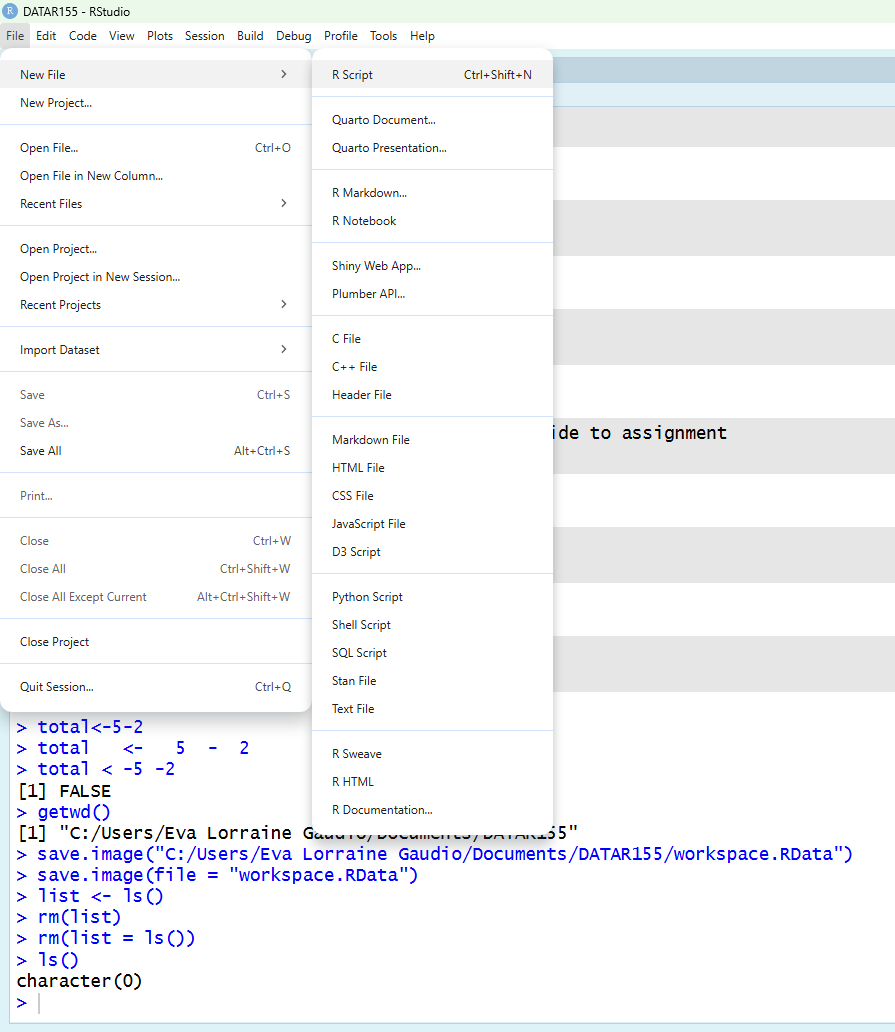
\includegraphics[keepaspectratio]{new_rscript.png}}
\caption{Figure 1. The RStudio Script Editor pane with a script open.}
\end{figure}

Method B. \textbf{Keyboard Shortcut}

\begin{enumerate}
\def\labelenumi{\arabic{enumi}.}
\tightlist
\item
  Use the keyboard shortcut Ctrl + Shift + N (or Cmd + Shift + N on a
  Mac).
\end{enumerate}

🎯 Open a new R Script.

\begin{Shaded}
\begin{Highlighting}[]
\CommentTok{\# Create a new script }
\end{Highlighting}
\end{Shaded}

🗣 An empty script opens in the Script Editor (also called the Source
pane).

\begin{Shaded}
\begin{Highlighting}[]
\CommentTok{\# ⚡ Type this in your R Script}
\NormalTok{six }\OtherTok{\textless{}{-}} \DecValTok{6}
\NormalTok{seven }\OtherTok{\textless{}{-}} \DecValTok{7}
\NormalTok{eight }\OtherTok{\textless{}{-}} \DecValTok{8}
\NormalTok{nine }\OtherTok{\textless{}{-}} \DecValTok{9}
\end{Highlighting}
\end{Shaded}

\section{Run Code}\label{run-code}

🎯 Place your cursor on each line and click Run (or press Ctrl+Enter on
Windows/Linux or Cmd+Return on macOS) to send that line to the Console
where it executes.

\begin{figure}
\centering
\pandocbounded{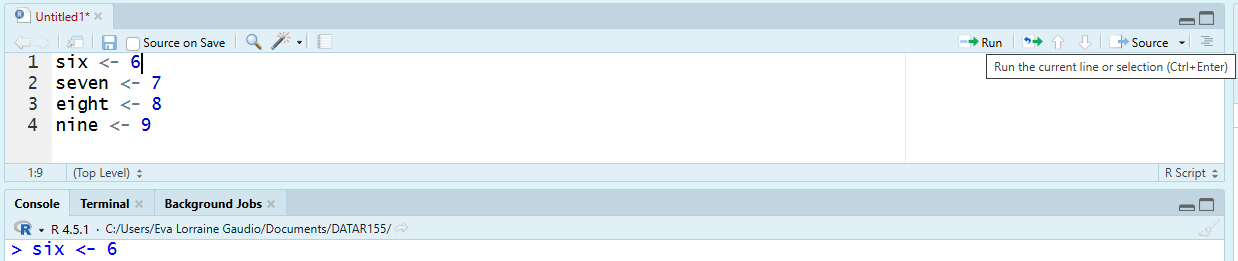
\includegraphics[keepaspectratio]{run_script.png}}
\caption{Figure 5. The RStudio Script Editor pane with a script open.}
\end{figure}

\begin{Shaded}
\begin{Highlighting}[]
\CommentTok{\# Run one line}
\end{Highlighting}
\end{Shaded}

🎯 Select multiple lines to run them together.

\begin{figure}
\centering
\pandocbounded{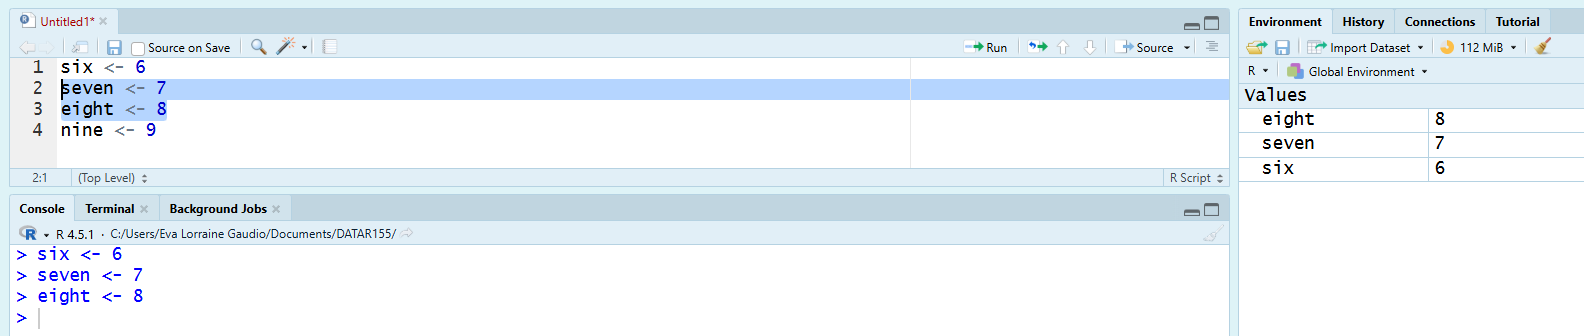
\includegraphics[keepaspectratio]{run_script2.png}}
\caption{Figure 2. The RStudio Script Editor pane with a script open.
Two lines are highlighted and both were run in the console using
Ctrl+Enter.}
\end{figure}

\begin{Shaded}
\begin{Highlighting}[]
\CommentTok{\# Run multiple lines at the same time}
\end{Highlighting}
\end{Shaded}

🎯 Click Source to run the entire script at once.

\begin{figure}
\centering
\pandocbounded{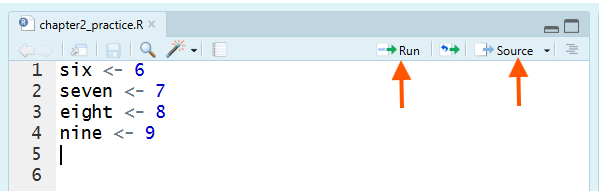
\includegraphics[keepaspectratio]{run_source.png}}
\caption{Figure 3. The RStudio Script Editor pane with a script open.}
\end{figure}

\begin{Shaded}
\begin{Highlighting}[]
\CommentTok{\# Source the entire script}
\end{Highlighting}
\end{Shaded}

\section{Save Your Script}\label{save-your-script}

Saving your R script preserves the instructions (your code and
comments), not the objects in your Environment. This matters because
when you restart R or switch computers your Environment can disappear.
Your script is a document of your work. A saved script lets anyone
re-run your code and reproduce your results.

Most assignments in this course will require that you submit file that
contains code and memos. Early modules require you submit an R script
file (\texttt{.R}). The .R extension helps RStudio (and your computer)
recognize the file as an R script.

There are two primary ways to save your script. You can use either
method.

Method A. \textbf{Save icon}

\begin{enumerate}
\def\labelenumi{\arabic{enumi}.}
\tightlist
\item
  Click the Save icon (floppy disk) in the toolbar of the Script Editor
  pane.
\end{enumerate}

\begin{figure}
\centering
\pandocbounded{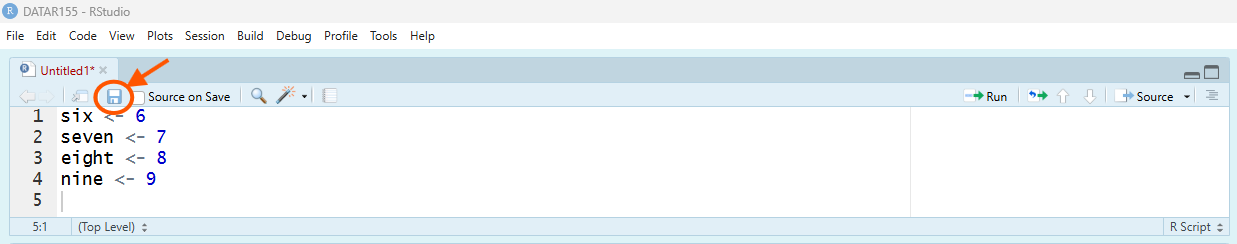
\includegraphics[keepaspectratio]{save_icon.png}}
\caption{Figure 4. The RStudio Script Editor pane with a script open.}
\end{figure}

Method B. \textbf{File Menu}

\begin{enumerate}
\def\labelenumi{\arabic{enumi}.}
\item
  Go to the File menu at the top left of RStudio.
\item
  Select Save As\ldots.
\end{enumerate}

\begin{Shaded}
\begin{Highlighting}[]
\CommentTok{\# Save your script in your course folder (e.g., Intro\_to\_R)}
\CommentTok{\# File name: chapter2\_notes}
\CommentTok{\# Save a type: R}
\end{Highlighting}
\end{Shaded}

\begin{quote}
🧐 \textbf{Notice:} that the file extension \texttt{.R} is automatically
added.
\end{quote}

\begin{Shaded}
\begin{Highlighting}[]
\CommentTok{\# ✅ Verify that \textasciigrave{}chapter2\_notes.R\textasciigrave{} is in the right folder.}
\end{Highlighting}
\end{Shaded}

💡 \textbf{Tip:} ``Working directory'' controls where R looks for files
when you use relative paths, but you can still accidentally save a
script somewhere else if you choose the wrong folder in the Save dialog.
For this course, always save scripts into your course folder so your
files stay together and you can find them when it's time to upload.

💡 \textbf{Tip:} When your script is unsaved, RStudio typically shows an
asterisk (*) in the script tab and the file name is red, which means you
have changes that are not saved yet.

\begin{center}\rule{0.5\linewidth}{0.5pt}\end{center}

📖 \textbf{Review}

Recall that objects are names that store elements in R. You can use
objects in calculations just like you would use numbers.

\begin{Shaded}
\begin{Highlighting}[]
\CommentTok{\# ⚡ Type this in your R Script}
\CommentTok{\# The Incident: Why is 6 afraid?}
\NormalTok{seven\_eight }\OtherTok{\textless{}{-}}\NormalTok{ seven }\SpecialCharTok{+}\NormalTok{ eight}

\CommentTok{\# The Result:}
\NormalTok{the\_aftermath }\OtherTok{\textless{}{-}}\NormalTok{ seven\_eight }\SpecialCharTok{{-}}\NormalTok{ nine}
\end{Highlighting}
\end{Shaded}

\begin{Shaded}
\begin{Highlighting}[]
\CommentTok{\# ✅ What number should be scared?}
\FunctionTok{print}\NormalTok{(the\_aftermath)}
\end{Highlighting}
\end{Shaded}

\begin{center}\rule{0.5\linewidth}{0.5pt}\end{center}

🎯 Run in order from top to bottom so that objects exist before you use
them.

\begin{Shaded}
\begin{Highlighting}[]
\CommentTok{\# Select and run in order}
\end{Highlighting}
\end{Shaded}

🛠 \textbf{Break Things!} Order matters when editing and running code
from a script.

Pretend that you decided to change the name of \texttt{seven\ +\ eight}
to \texttt{seven.eight}.

🎯 Edit your script.

\begin{Shaded}
\begin{Highlighting}[]
\CommentTok{\# Edit the object name}
\NormalTok{seven.eight }\OtherTok{\textless{}{-}}\NormalTok{ seven }\SpecialCharTok{+}\NormalTok{ eight}
\NormalTok{the\_aftermath }\OtherTok{\textless{}{-}}\NormalTok{ seven.eight }\SpecialCharTok{{-}}\NormalTok{ nine}
\end{Highlighting}
\end{Shaded}

Go back to your script and run ONLY \texttt{the\_aftermath} line
(without running the lines above it).

\begin{Shaded}
\begin{Highlighting}[]
\CommentTok{\# Run only this line}
\NormalTok{the\_aftermath }\OtherTok{\textless{}{-}}\NormalTok{ seven.eight }\SpecialCharTok{{-}}\NormalTok{ nine}
\end{Highlighting}
\end{Shaded}

✍️ Error: object `seven.eight' not found. 🗣 This is an error because
\texttt{seven.eight} has not been created yet in this session.

🚧 \textbf{Errors} prevent code from running.

🤔 No Error? This example may not error if you already ran
\texttt{seven.eight\ \textless{}-\ seven\ +\ eight} before
\texttt{the\_aftermath\ \textless{}-\ seven.eight\ -\ nine}. Another way
you can produce the error is by clearing the Environment before testing.
🧹 Sweep your environment and run code out of order.

💡 \textbf{Tip:} All scripts submissions must be able to run from top to
bottom without errors. Regularly test your script by clicking Source to
ensure that all lines run without errors.

In R, an error message is not a judgment. It is the computer telling you
exactly what it cannot do \emph{yet}. Learning to read errors calmly and
then adjusting your next step is a core part of learning to code.

\begin{center}\rule{0.5\linewidth}{0.5pt}\end{center}

Next, you will learn how to use comments as memos to document when you
encounter errors.

\chapter{Memo in R Scripts}\label{memo-in-r-scripts}

To add comments in an R script, simply use the ``\#'' symbol at the
beginning of a line to indicate that the following text is a comment and
should be ignored by the R interpreter.

You can add a line break to a long comment by using the \# symbol on
each new line. This is necessary because R interprets everything on a
single line after the first \# as part of the comment. For example:

\begin{Shaded}
\begin{Highlighting}[]
\CommentTok{\# This is a comment. Notice the "\#" at the beginning of the line.}

\CommentTok{\# Comments often explain something about the code or your thinking.}
\CommentTok{\# You will create comments like this in R Script assignments to }
\CommentTok{\#  document your process.}

\CommentTok{\# Break the comment into several lines to keep the message readable.}
\end{Highlighting}
\end{Shaded}

\section{Explain Your Thinking}\label{explain-your-thinking}

Researchers have found that typing self-explanations of code improves
retention and deepens understanding (Rus et. al., 2021). As you work
through exercises and assignments, document a running record of
insights, hunches, hypotheses, discussions about the applications of the
code.

\begin{enumerate}
\def\labelenumi{\arabic{enumi}.}
\item
  \textbf{Forethought} before action. Before running code, write a brief
  note about the 🎯 Goal of code should accomplish, 💬 Prediction of
  what you expect to happen, or identify your 🧠 motivational beliefs
  that support persistence.
\item
  \textbf{Performance} monitoring during action. ⚡ Compose the code and
  ✅ Check that the code worked. 🚀 Conduct Code trials, debugging
  issues, and ✍️ keep a record what you tried, even if it didn't work.
\item
  \textbf{Self-reflection} after action. After getting the code to work,
  🗣 Comment about what you learned, what surprised you, or what
  questions remain. 🪞 Reflect on learning process and what you will do
  next time.
\end{enumerate}

Icons for these strategies are provided in throughout each chapter to
model the process. Mirror this process in all work you submit for the
course. Each chapter will highlight specific memoing practices to focus
on. This chapter focuses on documenting your tenacity.

\begin{center}\rule{0.5\linewidth}{0.5pt}\end{center}

Now that you know how to write and run code in a script, you will likely
encounter errors. Tenacity is the learning skill that helps you persist
through those errors and learn from them.

\chapter{Tenacity}\label{tenacity}

To successfully learn R programming, you will need to persist through
difficulties, revise code, and know when to seek help after genuine
effort. Tenacity is the learning skill that shows up when you persist
through obstacles (confusion, errors, frustration), revise your
approach, and know when to seek help after genuine effort rather than
quitting too early or grinding aimlessly (King, 2021; Baehr, 2022).
Tenacity is not ``never give up.'' It's productive persistence.

\section{Why R is Challenging}\label{why-r-is-challenging}

R is not hard because it's mysterious. It's hard because it's precise.
Small mistakes (a missing parenthesis, a comma in the wrong place, a
misspelled object name) produce errors, and those errors are not
personal---they're information.

You may have already encountered friction in exactly the places
beginners expect to be ``simple'':

\begin{itemize}
\item
  Installing or updating R/RStudio
\item
  Saving and submitting scripts and file to Canvas
\item
  Creating objects and then getting object not found errors
\end{itemize}

If you treat every error as evidence you ``can't code,'' you will stall.
Tenacity is what keeps you moving long enough for the patterns to become
familiar (King, 2021).

\section{Getting Stuck}\label{getting-stuck}

\textbf{Two Ways of Getting Stuck}

\begin{enumerate}
\def\labelenumi{\arabic{enumi})}
\tightlist
\item
  Giving up too early (irresolution).
\end{enumerate}

This looks like skipping checks, continuing ``halfway,'' or abandoning
the task the moment you feel lost (King, 2021). In R, that often
becomes: running code you don't understand, hoping it works, and
stacking confusion.

\begin{enumerate}
\def\labelenumi{\arabic{enumi})}
\setcounter{enumi}{1}
\tightlist
\item
  Pushing too long (intransigence).
\end{enumerate}

This looks like repeating the same approach for too long even though it
isn't working, refusing to change strategy, and refusing help (King,
2021). In R, that often becomes: re-running the same broken line 30
times.

Tenacity lives in the middle: persist, then recalibrate.

\section{Document Tenacity}\label{document-tenacity}

When you encounter a challenge, document your tenacity on a memo. Your
memo will show a running log of what you tried and how you resolved the
issue.

\subsection{✍️ Record what you tried}\label{record-what-you-tried}

Prevent future duplication of errors, contextualizing successes, and
exposes hidden discoveries (unanticipated effect) by recording your
learning process on a memo in your R script.

When you encounter an error:

\begin{enumerate}
\def\labelenumi{\arabic{enumi}.}
\item
  \textbf{Comment out the code line(s) that produced the error} by
  adding a \texttt{\#} at the beginning of the line. This is really
  important. You want to keep the code visible for reference, but your
  script must not produce an error.
\item
  \textbf{Copy and paste the error message} below the commented line.
\item
  \textbf{Comment out the error message} by adding a \texttt{\#} at the
  beginning of each line.
\item
  \textbf{Add a brief comment explaining} what you think caused the
  error or how you will resolve it. This can come from your own
  reasoning or from external resources you consulted (peers,
  instructors, online resources, AI tools, etc.). Be sure to cite any
  resources you used. See the \textbf{Cite Your Resources} section below
  for guidance.
\item
  On a new line, compose the code that you believe will run without
  error. If the error is not yet resolved, repeat this listed process
  until you get the code to run without error.
\end{enumerate}

\begin{center}\rule{0.5\linewidth}{0.5pt}\end{center}

🧩 \textbf{Memo Example}

Below is a common beginner error along with memos documenting the
tenacity process.

\begin{Shaded}
\begin{Highlighting}[]
\CommentTok{\# 🧩 Example 1}
\CommentTok{\# 3.008+7*24)}
\CommentTok{\# Error: unexpected \textquotesingle{})\textquotesingle{} in "3.008+7*24)"}
\CommentTok{\# memo: This error is because the ) is a typo. }
\FloatTok{3.008}\SpecialCharTok{+}\DecValTok{7}\SpecialCharTok{*}\DecValTok{24}
\end{Highlighting}
\end{Shaded}

\begin{quote}
🧐 \textbf{Notice:} The student (1) ✍️ kept but commented out
(\texttt{\#}) the code with the error, (2) ✍️ copied and pasted the
error from the console, (3) 🗣 composed a memo that recognized the
unexpected parenthesis as a typo and (4) ⚡ composed new code that
removed it to fix the error.
\end{quote}

\emph{Memo examples like this one are provided throughout the each
chapter.}

\begin{center}\rule{0.5\linewidth}{0.5pt}\end{center}

💡 \textbf{Tip:} You can quickly comment/uncomment selected lines with
Ctrl+Shift+C (Windows/Linux) or Cmd+Shift+C (macOS).

\section{👀 Cite Your Resources}\label{cite-your-resources}

R syntax can be challenging, unforgiving even. Students often spend
hours debugging simple issues. Knowing how R interprets your code helps
avoid mistakes. Errors are usually simple but hard to spot alone. That's
normal.

Before you seek help, document three things in your script memo:

\begin{enumerate}
\def\labelenumi{\arabic{enumi}.}
\item
  🎯 What you what you were trying to do,
\item
  ⚡ The attempts at writing the code️ even if it didn't achieve the
  results you wanted.
\item
  ✍ State what you understand so far, and what you're confused or
  curious about.
\end{enumerate}

Once you decide to seek help, choose a resource that fits the problem: a
peer, your instructor, R's help files, reputable online documentation,
or an AI tool. No matter what you use, cite it in your memo so your
learning is traceable and your work is honest.

In your script, always include:

\begin{enumerate}
\def\labelenumi{\arabic{enumi}.}
\item
  \textbf{Who/what helped you} (person, website, help file, AI tool,
  etc.).
\item
  \textbf{How it helped you} (what you changed, what you learned, what
  you verified).
\end{enumerate}

Always write your own code; do not copy and paste from external sources.
Use external help to understand and learn, not to complete assignments
for you.

💡 \textbf{Tip:} If you use generative AI to help you and it provides
the answer, close the viewer and type the script yourself.

🧩 \textbf{Memo Example}

\begin{Shaded}
\begin{Highlighting}[]
\CommentTok{\# 🧩 Example 2}
\CommentTok{\# logicals2 \textless{}{-} c( 1\textgreater{}2, 3\textless{}5, 4=4 )}
\CommentTok{\# error: Error: unexpected \textquotesingle{}=\textquotesingle{} in "logicals2 \textless{}{-} c( 1\textgreater{}2, 3\textless{}5, 4="}
\NormalTok{logicals2 }\OtherTok{\textless{}{-}} \FunctionTok{c}\NormalTok{( }\DecValTok{1}\SpecialCharTok{\textgreater{}}\DecValTok{2}\NormalTok{, }\DecValTok{3}\SpecialCharTok{\textless{}}\DecValTok{5}\NormalTok{, }\DecValTok{4}\SpecialCharTok{==}\DecValTok{4}\NormalTok{ )}
\CommentTok{\# memo: I remember the instruction video but wanted to test what kind of error it would show.}
\CommentTok{\# memo: I noticed that under value "logicals2" in the environment" it has answered whether or not my equations are true or false}
\NormalTok{logicals2}
\CommentTok{\# memo: Here\textquotesingle{}s what came back in the console! [1] FALSE  TRUE  TRUE}
\CommentTok{\# memo: That means 1\textgreater{}2 is false, 3\textless{}5 is true, and 4=4 is true}
\end{Highlighting}
\end{Shaded}

\begin{quote}
🧐 \textbf{Notice:} The student (1) ✍️ kept but commented out
(\texttt{\#}) the code with the errors, (2) ✍️ copied and pasted the
error shown in the console, (3) 👀 cites a course video and the intent
to 🛠 \textbf{Break Things!} to understand errors, (4) ⚡ revised the
code to fix the errors, and 🗣 explained the final results.
\end{quote}

\begin{center}\rule{0.5\linewidth}{0.5pt}\end{center}

We turn to building basic objects next. As you work through the
exercises, practice documenting your tenacity on a memo whenever you
encounter an error or do not fully understand.

\begin{center}\rule{0.5\linewidth}{0.5pt}\end{center}

\chapter{Vectors}\label{vectors}

So far, we have only stored single numbers in objects. These
single-element numeric objects are often called \textbf{scalars}. R can
also store collections of values in a single object.

\begin{Shaded}
\begin{Highlighting}[]
\CommentTok{\# ⚡ Type this in your R Script}
\NormalTok{scalar }\OtherTok{\textless{}{-}} \DecValTok{42}
\end{Highlighting}
\end{Shaded}

An \textbf{atomic vector} one-dimensional object that stores an ordered
collection of values (\textbf{elements}), all of the same basic type.
For simplicity, I will simply use the word \textbf{vector}. A vector is
like a row in a spreadsheet: a single dimension of related values.

Let's use \texttt{c()}, \texttt{:}, and \texttt{seq()} to create vectors
of different storage types: numeric, integer, and character.

\section{\texorpdfstring{Numeric Vectors with
\texttt{c()}}{Numeric Vectors with c()}}\label{numeric-vectors-with-c}

\textbf{Numeric vectors} are a list of numbers. So far, we have only
stored single numbers in objects.

Vector Method A. Use the \texttt{c()} function to combine (or
``\textbf{concatenate}'') values into a single vector.

🎯 Create a numeric vector named \texttt{numbers3} that contains three
decimal point and negative numbers using the \texttt{c()} function.

\begin{Shaded}
\begin{Highlighting}[]
\CommentTok{\# ⚡ Type this (or something similar) in your R Script}
\NormalTok{numbers3  }\OtherTok{\textless{}{-}} \FunctionTok{c}\NormalTok{(}\FloatTok{1.5}\NormalTok{, }\FloatTok{2.5}\NormalTok{, }\SpecialCharTok{{-}}\FloatTok{3.5}\NormalTok{)                }\CommentTok{\# Numeric with decimals and negative}
\end{Highlighting}
\end{Shaded}

\begin{Shaded}
\begin{Highlighting}[]
\CommentTok{\# ✅ Check that numbers3 was created }
\FunctionTok{print}\NormalTok{(numbers3)}
\end{Highlighting}
\end{Shaded}

🗣 The output shows the three numbers stored in the \texttt{numbers3}
vector.

\begin{quote}
🧐 \textbf{Notice:} You can see object details by looking at the
Environment pane. The \texttt{numbers3} object shows as ``num
{[}1:3{]}'' indicating it is a numeric vector with three elements. These
numbers are ``numeric'' because they include decimal points. The
placement of the numbers in the list is ordered exactly as you entered
them.
\end{quote}

\section{\texorpdfstring{Integer Vectors with
\texttt{c()}}{Integer Vectors with c()}}\label{integer-vectors-with-c}

\textbf{Integer vectors} are a list of whole numbers. In R, integers are
typically written with an \texttt{L} suffix.

🎯 Create a vector named \texttt{cursed\_seq} that contains the integer
values 4, 8, 15, 16, 23, and 42 using the \texttt{c()} function.

\begin{Shaded}
\begin{Highlighting}[]
\CommentTok{\# ⚡ Type this in your R Script}
\NormalTok{cursed\_seq }\OtherTok{\textless{}{-}} \FunctionTok{c}\NormalTok{(}\DecValTok{4}\DataTypeTok{L}\NormalTok{, }\DecValTok{8}\DataTypeTok{L}\NormalTok{, }\DecValTok{15}\DataTypeTok{L}\NormalTok{, }\DecValTok{16}\DataTypeTok{L}\NormalTok{, }\DecValTok{23}\DataTypeTok{L}\NormalTok{, }\DecValTok{42}\DataTypeTok{L}\NormalTok{)          }\CommentTok{\# Integer via c()}
\end{Highlighting}
\end{Shaded}

\begin{Shaded}
\begin{Highlighting}[]
\CommentTok{\# ✅ Check that cursed\_seq was  created}
\FunctionTok{print}\NormalTok{(cursed\_seq)}
\end{Highlighting}
\end{Shaded}

🗣 The output shows the integer values stored in the \texttt{cursed\_seq}
vector. 🎬 Optional aside: Don't get \emph{Lost} with these numbers that
aren't a perfect mathematical progression.

\section{\texorpdfstring{Sequences with
\texttt{:}}{Sequences with :}}\label{sequences-with}

``\texttt{:}'' creates a simple sequence.

🎯 Create a numeric vector named \texttt{combination} that contains the
integer values from 1 to 5 using the \texttt{:} operator.

\begin{Shaded}
\begin{Highlighting}[]
\CommentTok{\# ⚡ Type this in your R Script}
\NormalTok{combination }\OtherTok{\textless{}{-}} \DecValTok{1}\SpecialCharTok{:}\DecValTok{5}                             \CommentTok{\# integer via :}
\end{Highlighting}
\end{Shaded}

\begin{Shaded}
\begin{Highlighting}[]
\CommentTok{\# ✅ Check that combination contains 1, 2, 3, 4, and 5 in order.}
\FunctionTok{print}\NormalTok{(combination)}
\end{Highlighting}
\end{Shaded}

🗣 The output shows 1 2 3 4 5 in order. 🎬 Optional aside: 1, 2, 3, 4, 5?
That's amazing! I've got the same combination on my luggage. (Yes, it's
a famous movie joke. Ignore it if you don't recognize it.)

\begin{enumerate}
\def\labelenumi{\arabic{enumi}.}
\setcounter{enumi}{2}
\tightlist
\item
  Vector Method C. Use \texttt{seq()} for custom steps.
\end{enumerate}

📜 The SYNTAX (basic):

\texttt{seq(from\ =\ 1,\ to\ =\ 10,\ by\ =\ 1)}

🎯 Create a numeric vector named \texttt{travel\_jumps} that contains
the numbers from 1887 to 2052 with steps of 33 using the \texttt{seq()}
function.

\begin{Shaded}
\begin{Highlighting}[]
\CommentTok{\# ⚡ Type this in your R Script}
\NormalTok{travel\_jumps }\OtherTok{\textless{}{-}} \FunctionTok{seq}\NormalTok{(}\AttributeTok{from =} \DecValTok{1887}\NormalTok{, }\AttributeTok{to =} \DecValTok{2052}\NormalTok{, }\AttributeTok{by =} \DecValTok{33}\NormalTok{)   }\CommentTok{\# numeric via seq()}
\end{Highlighting}
\end{Shaded}

\begin{Shaded}
\begin{Highlighting}[]
\CommentTok{\# ✅ Check that travel\_jumps contains the correct sequence.}
\FunctionTok{print}\NormalTok{(travel\_jumps)}
\end{Highlighting}
\end{Shaded}

🗣 The output shows the sequence of numbers stored in the
\texttt{travel\_jumps} vector. 🎬 Optional aside: Everything is
connected. Everything is built on the number 33. It's Dark.

\section{\texorpdfstring{Character Vectors with
\texttt{c()}}{Character Vectors with c()}}\label{character-vectors-with-c}

\textbf{Character vectors} store text strings, which are sequences of
characters enclosed in quotes. Character vectors can include letters,
numbers, symbols, and spaces. They are often used to represent names,
labels, or any other textual data.

Quotes are enclosed in either double quotes \texttt{"} or single quotes
\texttt{\textquotesingle{}}. Both types of quotes function the same way
in R, but it's important to be consistent within a single string. The
commas separate individual strings within the vector is outside the
quotes.

🎯 Create a character vector named \texttt{activation\_code} that
contains the following words: Longing, Rusted, Seventeen, Daybreak,
Furnace, Nine, Benign, Homecoming, One, and Freight Car using the
\texttt{c()} function.

\begin{Shaded}
\begin{Highlighting}[]
\CommentTok{\# ⚡ Type this in your R Script}
\NormalTok{activation\_code }\OtherTok{\textless{}{-}} \FunctionTok{c}\NormalTok{(}\StringTok{"Longing"}\NormalTok{, }\StringTok{"Rusted"}\NormalTok{, }\StringTok{"Seventeen"}\NormalTok{, }\StringTok{"Daybreak"}\NormalTok{, }\StringTok{"Furnace"}\NormalTok{, }\StringTok{"Nine"}\NormalTok{, }\StringTok{"Benign"}\NormalTok{, }\StringTok{"Homecoming"}\NormalTok{, }\StringTok{"One"}\NormalTok{, }\StringTok{"Freight Car"}\NormalTok{)}
\end{Highlighting}
\end{Shaded}

\begin{Shaded}
\begin{Highlighting}[]
\CommentTok{\# ✅ Check the activation\_code vector}
\FunctionTok{print}\NormalTok{(activation\_code)}
\end{Highlighting}
\end{Shaded}

🗣 The output shows the ten words stored in the \texttt{activation\_code}
character vector. 🎬 Optional aside: Ready to comply? Does this
word-list makes the example memorable?

R recognizes colors in character vectors.

🎯 Create a character vector named \texttt{rainbow} that contains the
color names of the rainbow using the \texttt{c()} function.

\begin{Shaded}
\begin{Highlighting}[]
\CommentTok{\# ⚡ Type this in your R Script}
\NormalTok{rainbow }\OtherTok{\textless{}{-}} \FunctionTok{c}\NormalTok{(}\StringTok{"red"}\NormalTok{, }\StringTok{"orange"}\NormalTok{, }\StringTok{"yellow"}\NormalTok{, }\StringTok{"green"}\NormalTok{, }\StringTok{"blue"}\NormalTok{,  }\StringTok{"violet"}\NormalTok{)}
\end{Highlighting}
\end{Shaded}

\begin{Shaded}
\begin{Highlighting}[]
\CommentTok{\# ✅ Check the rainbow vector}
\FunctionTok{print}\NormalTok{(rainbow)}
\end{Highlighting}
\end{Shaded}

🗣 The output shows the color names stored in the \texttt{rainbow}
character vector.

\section{Adding Elements to Vectors}\label{adding-elements-to-vectors}

You can add to the end of a vector using the \texttt{c()} function.

🎯 Add the color ``indigo'' to the end of the existing \texttt{rainbow}
vector.

\begin{Shaded}
\begin{Highlighting}[]
\CommentTok{\# ⚡ Type this in your R Script}
\NormalTok{rainbow\_plus }\OtherTok{\textless{}{-}} \FunctionTok{c}\NormalTok{(rainbow, }\StringTok{"indigo"}\NormalTok{)}
\end{Highlighting}
\end{Shaded}

\begin{Shaded}
\begin{Highlighting}[]
\CommentTok{\# ✅ Check the rainbow\_plus vector}
\FunctionTok{print}\NormalTok{(rainbow\_plus)}
\end{Highlighting}
\end{Shaded}

🗣 The output shows the new object \texttt{rainbow\_plus} vector with
``indigo'' added to the end.

\section{Logical Vectors}\label{logical-vectors}

\textbf{Logical vectors} are used for conditions and comparisons. They
contain TRUE or FALSE values.

🎯 Create a logical vector named \texttt{logicals} that contains the
values TRUE, FALSE, and NA using the \texttt{c()} function.

\begin{Shaded}
\begin{Highlighting}[]
\CommentTok{\# ⚡ Type this in your R Notebook}
\NormalTok{logicals }\OtherTok{\textless{}{-}} \FunctionTok{c}\NormalTok{(}\ConstantTok{FALSE}\NormalTok{, }\ConstantTok{TRUE}\NormalTok{, }\ConstantTok{TRUE}\NormalTok{, }\ConstantTok{FALSE}\NormalTok{, }\ConstantTok{TRUE}\NormalTok{, }\ConstantTok{TRUE}\NormalTok{, }\ConstantTok{TRUE}\NormalTok{, }\ConstantTok{TRUE}\NormalTok{, }\ConstantTok{TRUE}\NormalTok{, }\ConstantTok{NA}\NormalTok{)}
\end{Highlighting}
\end{Shaded}

\begin{Shaded}
\begin{Highlighting}[]
\CommentTok{\# ✅ Check the logicals vector}
\FunctionTok{print}\NormalTok{(logicals)}
\end{Highlighting}
\end{Shaded}

🗣 The output shows the logical values stored in the \texttt{logicals}
vector.

\begin{center}\rule{0.5\linewidth}{0.5pt}\end{center}

In the next section, you will learn how to inspect vectors to confirm
what they are before using them in your analysis.

\chapter{Inspecting Vectors}\label{inspecting-vectors}

Before using data, we need to confirm \emph{what} it is.

\section{Mode of a Vector}\label{mode-of-a-vector}

The storage type of a vector tells R how to interpret the data inside
it. The \texttt{mode()} function tells you what kind of data the object
is fundamentally made of. For typical vectors, the mode could be
``numeric,'' ``character,'' or ``logical'' to name a few.

\emph{The function} \texttt{typeof()} \emph{returns R's internal storage
type of an object. For a higher-level understanding of the data type, we
use the} \texttt{mode()} \emph{function.}

🎯 Use the \texttt{mode()} function to check the data type of the
\texttt{activation\_code} vector.

\begin{Shaded}
\begin{Highlighting}[]
\CommentTok{\# ⚡ Type this in your R Script}
\FunctionTok{mode}\NormalTok{(activation\_code)}
\end{Highlighting}
\end{Shaded}

🗣 The output shows that the \texttt{activation\_code} vector is of mode
``character,'' indicating it stores text.

🚀 \textbf{Explore and Play:} Try checking the mode of other vectors you
created, such as \texttt{numbers3}, \texttt{cursed\_seq},
\texttt{combination}, \texttt{travel\_jumps}, and \texttt{logicals}.

\begin{Shaded}
\begin{Highlighting}[]
\CommentTok{\# Check the mode of other vectors in your R Script}
\end{Highlighting}
\end{Shaded}

\section{Length of a Vector}\label{length-of-a-vector}

\texttt{length()} counts elements.

🎯 Use the \texttt{length()} function to find the number of elements in
the \texttt{activation\_code} vector.

\begin{Shaded}
\begin{Highlighting}[]
\CommentTok{\# ⚡ Type this in your R Script}
\FunctionTok{length}\NormalTok{(activation\_code)}
\end{Highlighting}
\end{Shaded}

🗣 The output shows the number of elements in the
\texttt{activation\_code} vector, which is 10.

🚀 \textbf{Explore and Play:} Try checking the length of other vectors
you created, such as \texttt{numbers3}, \texttt{cursed\_seq},
\texttt{combination}, \texttt{travel\_jumps}, and \texttt{logicals}.

\begin{Shaded}
\begin{Highlighting}[]
\CommentTok{\# Check the length of other vectors in your R Script}
\end{Highlighting}
\end{Shaded}

\chapter{Dataframes}\label{dataframes}

A \textbf{data frame} is a two-dimensional, tabular data structure in R
that can store data of different types (numeric, character, logical,
etc.) in each column. It is similar to a spreadsheet or SQL table and is
widely used for data analysis and manipulation in R.

We can create a data frame by combining multiple vectors of the
\emph{same length} using the \texttt{data.frame()} function.

📜 The SYNTAX (basic):

\texttt{data.frame(column1\ =\ c(...),\ column2\ =\ c(...),\ ...)}

🎯 Use vectors created earlier to build a data frame. We'll combine
vectors in the global environment that have the length of 6 elements.

\begin{Shaded}
\begin{Highlighting}[]
\CommentTok{\# ✅  Review Vectors }
\FunctionTok{print}\NormalTok{(rainbow)}
\FunctionTok{print}\NormalTok{(travel\_jumps)}
\FunctionTok{print}\NormalTok{(cursed\_seq)}
\end{Highlighting}
\end{Shaded}

\begin{Shaded}
\begin{Highlighting}[]
\CommentTok{\# ⚡ Type this in your R Script}
\CommentTok{\# Create the Data Frame}
\NormalTok{spectrum\_shift }\OtherTok{\textless{}{-}} \FunctionTok{data.frame}\NormalTok{(}
  \AttributeTok{Vibe =}\NormalTok{ rainbow,}
  \AttributeTok{Year =}\NormalTok{ travel\_jumps,}
  \AttributeTok{Code =}\NormalTok{ cursed\_seq}
\NormalTok{)}
\end{Highlighting}
\end{Shaded}

\begin{Shaded}
\begin{Highlighting}[]
\CommentTok{\# ✅ Check the spectrum\_shift Data Frame}
\FunctionTok{print}\NormalTok{(spectrum\_shift)}
\end{Highlighting}
\end{Shaded}

🗣 The output shows the \texttt{spectrum\_shift} data frame with three
columns: \texttt{Vibe}, \texttt{Year}, and \texttt{Code}. Each column
corresponds to one of the vectors we combined.

\begin{center}\rule{0.5\linewidth}{0.5pt}\end{center}

\chapter{Summary}\label{summary}

This chapter taught you how to work in an R script: create a new
\texttt{.R} file in the Source pane, run code into the Console with
RStudio's Run commands/shortcuts, and use comments to document what you
tried when something failed. You built vectors with \texttt{c()},
\texttt{:} and \texttt{seq()}, practiced element-wise vector arithmetic
(including R's recycling behavior and the warnings it can trigger),
created character and logical vectors, and then checked objects with
\texttt{mode()} and \texttt{length()} to confirm what they are before
using them. Finally, you combined same-length vectors into a data frame
using \texttt{data.frame()}, which is the standard ``table'' structure
you will use constantly in later chapters.

\chapter{Chapter Terms}\label{chapter-terms}

\textbf{Atomic Vector}: A one-dimensional R vector where all elements
must be the same basic type (logical, integer, double/numeric,
character, complex, or raw). If you combine different types, R will
coerce them to a single type so the vector stays atomic.

\textbf{Character Vector}: A vector that stores text strings, written in
quotes, such as \texttt{"apple",\ "banana",\ "grapes"} or
\texttt{"ID\_001",\ "ID\_002",\ "ID\_003"}.

\textbf{Concatenate} \texttt{c()}: A function that combines
(concatenates) values into a single vector. You use \texttt{c()} to
create a vector, append items to an existing vector, or join multiple
vectors together (for example, \texttt{c(1,\ 2,\ 3)} or
\texttt{c(x,\ y))}.

\textbf{Data Frame}: A rectangular table-like object where each column
is a vector (all values in a column share the same type), and all
columns have the same number of rows. Data frames are the standard
structure for working with datasets in R because they organize variables
(columns) and observations (rows) in a consistent format.

\textbf{Elements}: The individual data values stored inside a vector
object. Each element has a position (its index) and can be accessed by
indexing (for example, \texttt{x{[}1{]}} for the first element).

\textbf{Error}: A console message indicating that R could not complete a
command. Execution stops at that point, no result is produced for that
step, and you must fix the problem (for example, a misspelled object
name, invalid argument, or syntax issue) before the code can run.

\textbf{File Menu}: The top-left menu in RStudio that provides commands
for creating, opening, saving, exporting, and printing files and
projects. It's where you start new items (for example, a new R Script),
open existing files, manage recent files/projects, and access
project-level actions.

\textbf{Hexadecimal Color Codes}: A way to specify colors using a
\texttt{\#} followed by hexadecimal digits. In R (and most software),
\texttt{\#RRGGBB} defines the red, green, and blue intensities using two
hex digits each (00--FF), for example \texttt{\#FF0000} (red) or
\texttt{\#1E90FF} (blue). Some codes include transparency as a fourth
pair, \texttt{\#RRGGBBAA}, where \texttt{AA} controls alpha (00 = fully
transparent, FF = fully opaque).

\textbf{Integer Vector}: A vector that stores whole numbers. In R,
integers are typically written with an \texttt{L} suffix, such as
\texttt{1L} or \texttt{42L}.

\textbf{Length} \texttt{length()}: A function that returns the number of
elements in an object. For a vector, \texttt{length(x)} is the count of
elements in the vector; for a list, it's the number of list components;
for a data frame, it returns the number of columns.

\textbf{Mode}: The underlying storage type of an R object---the
low-level kind of data it is fundamentally stored as. \texttt{mode(x)}
reports this storage mode (often aligning with atomic types like
\texttt{"numeric"}, \texttt{"integer"}, \texttt{"logical"}, or
\texttt{"character"}), which is useful for understanding coercion and
how R will treat the object in computations.

\textbf{Numeric Vector}: A vector that stores real (decimal) numbers,
such as \texttt{3.14}, \texttt{-2.5}, or \texttt{0}.

\textbf{Recycling}: R's rule for handling vector operations when the
vectors have different lengths. The shorter vector is repeated
(recycled) to match the length of the longer vector, then the operation
is performed element-by-element. Recycling is safe only when the longer
length is an exact multiple of the shorter; otherwise R issues a warning
and the result may be unreliable.

\textbf{R Script}: A plain-text file (typically saved with a \texttt{.R}
extension) that contains a sequence of R commands you write and save for
later use. An R script lets you run code in a repeatable, organized
way---so you can recreate analyses, clean data, define functions, and
document your workflow without relying on one-off console commands.

\textbf{Scalars}: Single-value objects (length 1). In R, scalars are not
a separate data type---what people call a ``scalar'' is typically an
atomic vector with exactly one element (numeric, character, logical,
etc.).

\textbf{Vector}: A one-dimensional object that stores an ordered
sequence of elements of the same basic type (for example, all numeric,
all character, or all logical). Vectors are the core building block of
many R objects, and you create them with functions like \texttt{c()};
you can subset them by position or by logical conditions.

\textbf{Vector Arithmetic}: Performing mathematical operations directly
on vectors. In R, operations like\texttt{+}, \texttt{-}, \texttt{*},
\texttt{/}, and \texttt{\^{}} are applied element-by-element, so
\texttt{c(1,\ 2,\ 3)\ +\ c(10,\ 20,\ 30)} returns
\texttt{c(11,\ 22,\ 33)}.

\textbf{Warning}: A console message indicating that R did run the
command but detected a potential problem. Execution continues and a
result is produced, but the output may be incomplete, unexpected, or
based on an assumption (for example, coercing types, removing missing
elements, or using a function in a way that may not behave as intended).

\chapter{📝 Practice Space}\label{practice-space}

Fill in the blanks to complete the code in your R Script.

Before you begin:

\begin{enumerate}
\def\labelenumi{\arabic{enumi}.}
\tightlist
\item
  Create a new R Script in RStudio.
\item
  Save it in your course folder as \texttt{chapter2\_practice.R}.
\item
  Complete all Practice Space tasks in that notebook.
\item
  Save your workspace as \texttt{chapter2\_practice.RData}.
\end{enumerate}

Required files to submit:

\begin{itemize}
\tightlist
\item
  \texttt{chapter2\_practice.R}
\item
  \texttt{chapter2\_practice.RData}
\end{itemize}

As you work, add short comments or memo notes explaining what your code
is doing and what the output shows.

If you encounter an error, document your \textbf{tenacity} by briefly
noting what happened, what you tried, and how you fixed it or what still
confuses you.

Before submitting, clear your Environment and run the notebook from top
to bottom. Objects need to be created in sequential order.

All work must be hand-typed by you in your own voice. Do not copy and
paste from AI. You make quote AI output anywhere (clear quotation marks
or quote (\texttt{\textgreater{}}) before the paragraph). Hand-type a
explanation of why you're including that quote.

\section{Task 0}\label{task-0}

Before you begin, make sure you have created a new R script in the
Source pane. Additionally, sweep your environment before running the
code. When you finish, be sure to source your entire script to ensure it
runs without errors from top to bottom.

Save your R script (\texttt{chapter2\_practice.R}) and environment
(\texttt{chapter2\_practice.RData}) in your course folder.

Remember to document your \textbf{tenacity} in a memo if you encounter
any errors while completing the tasks.

Save before closing RStudio. Submit to Canvas modules, as directed.

\section{Task 1}\label{task-1}

Type this in your R Script, Fill in the blanks

\begin{Shaded}
\begin{Highlighting}[]
\CommentTok{\# 🎯 Build a numeric vector named \textasciigrave{}exponents\textasciigrave{} that contains the numbers between 0.5 and 10 using the \textasciigrave{}seq()\textasciigrave{} function.}


\CommentTok{\# ⚡ }
\NormalTok{exponents }\OtherTok{\textless{}{-}} \FunctionTok{\_\_}\NormalTok{(}\AttributeTok{from =}\NormalTok{ \_, }\AttributeTok{to =}\NormalTok{ \_\_)}

\CommentTok{\# ✅ Check the exponents vector}
\FunctionTok{length}\NormalTok{(\_\_\_\_\_\_\_)}
\FunctionTok{mode}\NormalTok{(\_\_\_\_\_\_\_\_)}

\CommentTok{\# 🗣 Add Comment: "\# The output shows length \_ and mode \_\_\_\_."}
\end{Highlighting}
\end{Shaded}

\section{Task 2}\label{task-2}

Type this in your R Script, Fill in the blanks

\begin{Shaded}
\begin{Highlighting}[]
\CommentTok{\# 🎯 Create a numeric vector using \textasciigrave{}:\textasciigrave{} called \textasciigrave{}list\_numbers\textasciigrave{} that contains the **integer** values from 1 to 10.}


\CommentTok{\# ⚡}
\NormalTok{\_\_\_\_\_\_\_\_ }\OtherTok{\textless{}{-}}\NormalTok{ \_ \_ \_}

\CommentTok{\# ✅ Check the mode and length of the vector}
\FunctionTok{\_\_\_\_}\NormalTok{(list\_numbers)}
\FunctionTok{length}\NormalTok{(\_\_\_\_\_\_\_\_)}

\CommentTok{\# 🗣 Add Comment:  }
 
\CommentTok{\# The length is \_\_\_ elements (values).}
\CommentTok{\# The mode is \_\_\_\_\_\_\_\_.}
                 
\CommentTok{\# 🗣 Add Comment: How does \textasciigrave{}mode()\textasciigrave{} report integers and decimals?}
\end{Highlighting}
\end{Shaded}

\section{Task 3}\label{task-3}

R can store hexadecimal color codes in character vectors.
\textbf{Hexadecimal color} codes are six-digit codes that represent
colors in web design and digital graphics.

Type this in your R Script, Fill in the blanks

\begin{Shaded}
\begin{Highlighting}[]
\CommentTok{\# 🎯 Create a character vector named \textasciigrave{}nerdy\_palette\textasciigrave{} that contains the following hexadecimal color codes using the \textasciigrave{}c()\textasciigrave{} function.}

\CommentTok{\# ⚡ }
\NormalTok{\_\_\_\_\_\_ \_\_ }\FunctionTok{\_}\NormalTok{(}\StringTok{"\#7F00FF"}\NormalTok{, }\StringTok{"\#003B6F"}\NormalTok{, }\StringTok{"\#663399"}\NormalTok{, }\StringTok{"\#4F97A3"}\NormalTok{, }\StringTok{"\#FFF8E7"}\NormalTok{, }\StringTok{"\#000000"}\NormalTok{, }\StringTok{"\#03A062"}\NormalTok{, }\StringTok{"\#FF00FF"}\NormalTok{, }\StringTok{"\#CC0000"}\NormalTok{)}

\CommentTok{\# ✅ Count the number of elements in the nerdy\_palette vector }
\FunctionTok{\_\_\_\_\_\_}\NormalTok{(nerdy\_palette)}


\CommentTok{\# 🗣 Comment: The output shows there are \_\_ hexadecimal color code elements stored in the \textasciigrave{}nerdy\_palette\textasciigrave{} vector.}
\end{Highlighting}
\end{Shaded}

\section{Task 4}\label{task-4}

Type this in your R Script, Fill in the blanks

\begin{Shaded}
\begin{Highlighting}[]
\CommentTok{\# 🎯 Add "\#4D9E68" to the end of the existing \textasciigrave{}nerdy\_palette\textasciigrave{} vector.}


\CommentTok{\# ⚡}
\NormalTok{nerdy\_palette }\OtherTok{\textless{}{-}} \FunctionTok{c}\NormalTok{(\_\_\_\_, \_\_\_\_)}

\CommentTok{\# ✅ Check the number of elements in the nerdy\_palette vector}
\FunctionTok{length}\NormalTok{(\_\_\_\_)}
\FunctionTok{print}\NormalTok{(\_\_\_\_)}


\CommentTok{\# 🗣 Comment: The output shows the updated \textasciigrave{}nerdy\_palette\textasciigrave{} vector with \_\_ elements added to the \_\_\_(beginning, middle, or end).}
\end{Highlighting}
\end{Shaded}

\section{Task 5}\label{task-5}

Type this in your R Script, Fill in the blanks

\begin{Shaded}
\begin{Highlighting}[]
\CommentTok{\# 🎯 Create a vector named \textasciigrave{}color\_names\textasciigrave{} that contains the following names: "Octarine," "TARDIS Blue," "Rebeccapurple," "Hooloovoo," "Cosmic Latte," "Vantablack," "Matrix Green," "Source Engine Magenta," "Command Red," and "Impossible Green." Use the \textasciigrave{}c()\textasciigrave{} function.}

\CommentTok{\# ⚡ }
\NormalTok{color\_names \_\_  }\FunctionTok{\_\_}\NormalTok{(\_\_\_\_\_\_\_ \_\_\_\_\_\_\_ \_\_\_\_\_\_\_ \_\_\_\_\_\_\_ \_\_\_\_\_\_\_ \_\_\_\_\_\_\_ \_\_\_\_\_\_\_ \_\_\_\_\_\_\_ \_\_\_\_\_\_\_ \_\_\_\_\_\_\_)}

\CommentTok{\# ✅ Check the number of elements in the color\_names vector}
\FunctionTok{length}\NormalTok{(\_\_\_\_\_\_\_\_)}


\CommentTok{\# 🗣 Comment: The output shows the \_\_ color names stored in the \textasciigrave{}color\_names\textasciigrave{} character vector.}
\end{Highlighting}
\end{Shaded}

\section{Task 6}\label{task-6}

Type this in your R Script, Fill in the blanks

\begin{Shaded}
\begin{Highlighting}[]
\CommentTok{\# 🎯 Create a vector named \textasciigrave{}origin\textasciigrave{} that contains "Discworld," "Doctor Who," "CSS/Web Development," "Hitchhiker\textquotesingle{}s Guide to the Galaxy," "Astronomy," "Material Science," "The Matrix," "Video Gaming," "Star Trek," and "Visual Perception." Use the \textasciigrave{}c()\textasciigrave{} function.}

\CommentTok{\# ⚡ }
\NormalTok{\_\_\_\_\_\_ \_\_ c\_}\StringTok{"Discworld"}\NormalTok{, }\StringTok{"Doctor Who"}\NormalTok{, }\StringTok{"CSS/Web Development"}\NormalTok{, }\StringTok{"Hitchhiker\textquotesingle{}s Guide to the Galaxy"}\NormalTok{, }\StringTok{"Astronomy"}\NormalTok{, }\StringTok{"Material Science"}\NormalTok{, }\StringTok{"The Matrix"}\NormalTok{, }\StringTok{"Video Gaming"}\NormalTok{, }\StringTok{"Star Trek"}\NormalTok{, }\StringTok{"Visual Perception"}\NormalTok{\_}

\CommentTok{\# ✅ Check the number of elements in the origin vector}
\FunctionTok{length}\NormalTok{(\_\_\_\_\_\_\_)}

\CommentTok{\# 🗣 Comment: The output shows the \_\_ origins stored in the \textasciigrave{}origin\textasciigrave{} character vector.}
\end{Highlighting}
\end{Shaded}

\section{Task 7}\label{task-7}

Type this in your R Script, Fill in the blanks

\begin{Shaded}
\begin{Highlighting}[]
\CommentTok{\# 🎯 Create a data frame using \textasciigrave{}data.frame()\textasciigrave{} named \textasciigrave{}nerdy\_df\textasciigrave{} that contains three columns: "Color" (\textasciigrave{}color\_names\textasciigrave{}), "Hex" (\textasciigrave{}nerdy\_palette\textasciigrave{}), and "Origin" (\textasciigrave{}origin\textasciigrave{}). }

\CommentTok{\# ⚡ Type this in your R Script, Fill in the blanks}
\NormalTok{nerdy\_df }\OtherTok{\textless{}{-}} \FunctionTok{\_\_\_\_\_\_}\NormalTok{(}
  \AttributeTok{\_\_\_\_\_\_ =}\NormalTok{ color\_names,}
\NormalTok{  Hex \_ nerdy\_palette,}
  \AttributeTok{Origin =}\NormalTok{ \_\_\_\_\_\_}
\NormalTok{)}

\CommentTok{\# ⚡ Type this in your R Script, Fill in the blanks}
\FunctionTok{print}\NormalTok{(\_\_\_\_\_\_)}


\CommentTok{\# 🗣 Comment: The output shows the \textasciigrave{}nerdy\_df\textasciigrave{} data frame with three columns: \_\_\_\_\_\_, \_\_\_\_\_\_, and \_\_\_\_\_\_. }
\end{Highlighting}
\end{Shaded}

\chapter{References}\label{references}

Baehr, Jason. 2022. Deep in Thought: A Practical Guide to Teaching for
Intellectual Virtues. Harvard Education Press.

King, N. L. (2021). The excellent mind: Intellectual virtues for
everyday life. Oxford University Press.

Rus, V., Akhuseyinoglu, K., Chapagain, J., \& Tamang, L. J. (2021).
Prompting for Free Self-Explanations Promotes Better Code Comprehension.
(CSEDM workshop, EDM 2021).

\bibliography{references.bib}

\end{document}
